%!TEX encoding = UTF-8 Unicode 
%!TEX TS-program = pdflatex

\documentclass[a4paper,12pt,italian]{article} 
\usepackage[utf8]{inputenc}
\usepackage{babel}
\usepackage[utf8]{inputenc} 
\usepackage[T1]{fontenc}
\usepackage{indentfirst}
\usepackage{hyperref}
\usepackage{upquote}

\usepackage{pdflscape}
\usepackage{tikz}

\usepackage{graphicx} 

\graphicspath{{./images/}}

\pagestyle{plain} 
\author{------  ----- \\
	-------- -- -----} 
\date{Politecnico di Milano \\
	Scuola di Ingegneria Industriale e dell'Informazione \\
	Corso di Ingegneria Informatica \\
	Sezione Prof. Fornaciari \\
	A.A. 2019/2020}
\title{Prova finale -- Progetto di reti logiche}

\begin{document}	
	\maketitle
	\newpage
	\tableofcontents
	\newpage
	
	% Analisi dei requisiti

\section{Introduzione}

Scopo della Prova Finale di Reti Logiche \`e implementare un encoder per Working Zones come descritto dalla specifica fornita. Per la realizzazione del progetto \`e stata utilizzata la fpga xc7a200tfbg484-1 nell'editor di Vivado Webpack 2019; la documentazione utilizzata per la realizzazione del progetto consiste nelle guide base di Vivado e di VHDL fornite dai docenti.

\subsection{Scelte progettuali}

Secondo la specifica definita, per la realizzazione del progetto sono stati utilizzati due registri per mantenere l'indirizzo da codificare e l'indirizzo della Working Zone analizzata al momento. Inoltre, si \`e deciso di mantenere un registro contatore per le operazioni effettuate, usato anche per comandare gli indirizzi cui accedere; in questo modo la gestione dell'accesso alla memoria \`e stato delegato al data path invece che alla macchina a stati finiti.

In base alle richieste sono anche state effettuate le seguenti scelte:
\begin{itemize}	
	\item Poich\'e non viene dichiarato che le WZ si trovino sempre in un ordine definito il circuito analizzer\`a tutti gli indirizzi prima di giungere alla conclusione di non appartenenza a nessuna WZ dell'indirizzo.
	
	\label{eccezione}\item Per quanto riguarda i valori non validi, il circuito dovr\`a considerare gli indirizzi di input come interi unsigned, quindi non sar\`a possibile inserire valori al di sotto di quelli considerati validi; se viene inserito un valore da codificare superiore a 127 il comportamento non dovr\`a differire da un'esecuzione normale, ma in caso di indirizzo non presente nelle WZ il MSB verr\`a sovrascritto dal WZ\_BIT, mantenendo quindi un comportamento consistente anche in casi eccezionali.
\end{itemize}

\subsection{Ottimizzazione con pipeline}

Per sfruttare al meglio la capacit\`a di parallelizzazione dell'hardware si \`e optato per una soluzione con una pipeline, cosicch\'e i moduli di gestione indirizzi, input e analisi (illustrati in seguito) potessero lavorare in contemporanea, riducendo notevolmente il tempo di esecuzione. A causa di questa scelta \`e stato per\`o necessario utilizzare un registro contatore per gestire l'offset tra i moduli.

Un esempio di esecuzione delle tre componenti in parallelo \`e mostrato in Figura \ref{pipeline}: una volta iniziata l'esecuzione il circuito richiede alla memoria prima l'indirizzo da codificare, quindi l'indirizzo della prima Working Zone. Da questo punto inizia l'esecuzione parallela a pieno regime, per cui avvengono contemporaneamente:
\begin{itemize}
	\item Analisi dell'appartenenza a una WZ;
	\item Caricamento della WZ successiva (se esiste);
	\item Richiesta di quella dopo ancora (se esiste).
\end{itemize}
Se l'analisi di appartenenza \`e positiva il sistema viene congelato e si procede all'output, altrimenti questo avviene una volta terminata l'analisi dell'ultima Working Zone.

\begin{figure}[t]
	\centering
	{\includegraphics[width=\textwidth,keepaspectratio]
		{pipeline.eps}}
	\caption{Esempio di funzionamento della pipeline per caricamento e analisi}
	\label{pipeline} 
\end{figure}
	
	% Sezione dell'architettura

\begin{landscape}
	\begin{figure}[ht]
		\centering
		{\includegraphics[height=\textheight,keepaspectratio]
			{data_path.eps}}
		\caption{Data Path}
		\label{datapath}
	\end{figure}
\end{landscape}
\section{Architettura}

% Sezione per illustrare il data path

\subsection{Data Path}
In Figura \ref{datapath} \`e mostrato il datapath; sono stati omessi i componenti utilizzati per il reset dei registri per favorire la leggibilit\`a.

Al fine di sfruttare al meglio la pipeline \`e stato suddiviso in 4 parti: 
\begin{itemize}
	\item Gestione indirizzi, per calcolare gli indirizzi di memoria cui accedere
	e mantenere un contatore;
	\item  Gestione input, per caricare nei registri i valori presenti in memoria;
	\item Analisi, per valutare l'appartenenza di un indirizzo a una WZ;
	\item Output, per gestire i segnali da inviare alla memoria.	
\end{itemize}

\subsubsection{Gestione degli indirizzi di memoria}

La gestione degli indirizzi cui accedere \`e realizzata con il registro \texttt{regnext} a 4 bit, che a inizio esecuzione viene inizializzato a 0 mentre alla memoria \`e richiesto l'indirizzo da codificare. In seguito, il registro inizia un ciclo di conteggio per poter accedere a tutte le celle di memoria contenenti gli indirizzi delle Working Zones e mantenere un contatore utile a gestire gli offset dati dalla pipeline.

Questo modulo \`e realizzato in VHDL con un process per realizzare \texttt{regnext} (compreso il sommatore collegato) e due costrutti \texttt{with/select} per i multiplexer in serie. Il valore di \texttt{o\_address} viene infine ricavato concatenando i dodici zeri meno significativi all'uscita dei multiplexer (per raggiungere i 16 bit degli indirizzi).

\subsubsection{Gestione degli input}

Per gestire i valori di input sono utilizzati due registri a 8 bit collegati a \texttt{i\_data}; il registro \texttt{regin} contiene l'indirizzo da codificare, mentre \texttt{regwz} l'indirizzo base della Working Zone in esame in questa fase (il cui numero corrisponde a \texttt{regnext}$ - 1$ per l'offset di pipeline).

La realizzazione in VHDL si compone semplicemente di due registri (realizzati con dei process) collegati all'input e attivati mai contemporaneamente.

\subsubsection{Analisi}
La fase di analisi si avvale infine del registro \texttt{regsub} a 8 bit (inizializzato a un valore arbitrario non significativo), che contiene la differenza tra l'indirizzo da codificare e l'indirizzo base della WZ; se questo valore \`e compreso o uguale tra 0 e 3 allora l'indirizzo fa parte della WZ e viene attivato il flag \texttt{is\_in} (che blocca il caricamento dei registri \texttt{regnext} e \texttt{regsub} per congelare il sistema).

Il codice di realizzazione si avvale di un process per calcolare e salvare il valore di \texttt{regsub}, e di una batteria di comparatori per determinare il valore di \texttt{is\_in}, ottenuto in modo combinatorio con un'espressione logica.

\subsubsection{Output}
Da un punto di vista di pipeline la fase di output pu\`o essere considerata unita a quella di analisi, poich\'e composta solo da reti combinatorie (si trovano quindi sulla stessa Working Zone). Utilizzando il valore di \texttt{is\_in} vengono selezionati i 7 bit meno significativi dell'output:
\begin{itemize}
	\item Se \texttt{is\_in} = 0, viene selezionato il valore di \texttt{regin};
	\item Se \texttt{is\_in} = 1, l'uscita risulta essere la concatenazione della WZ e della codifica one-hot del valore di \texttt{regsub}.
\end{itemize}
In quest'ultimo caso, il valore della Working Zone in uscita \`e determinato come i 3 bit meno significativi del valore (bloccato da \texttt{is\_in}) contenuto in \texttt{regnext}, cui viene sottratto l'offset dovuto al ritardo nella pipeline (ovvero 2 + 1 dovuto alla commutazione di \texttt{regnext}); la WZ \`e quindi \texttt{regnext}$ - 3$. Inoltre, \texttt{is\_in} stesso viene utilizzato come bit pi\`u significativo dell'output.
\begin{figure}[t]
	\centering	
	{\includegraphics[scale=0.7,keepaspectratio]
		{1hot.eps}}
	\caption{Encoder one-hot a due ingressi}
	\label{1hot} 
\end{figure}
La codifica one-hot a 2 ingressi \`e invece ottenuta attraverso una rete combinatoria (Illustrata in Figura \ref{1hot}) ricavata dalla seguente tavola di verit\`a:
\begin{center}
	\begin{tabular}{c c|c c c c}
		A & B & U3 & U2 & U1 & U0 \\
		\hline
		0 & 0 & 0 & 0 & 0 & 1 \\
		0 & 1 & 0 & 0 & 1 & 0 \\
		1 & 0 & 0 & 1 & 0 & 0 \\
		1 & 1 & 1 & 0 & 0 & 0
	\end{tabular}
\end{center}

La codifica VHDL del modulo viene realizzata con un costrutto \texttt{with/select} per il multiplexer (per cui uno degli ingressi risulta essere la concatenazione del valore della WZ attuale e dell'uscita dell'encoder one hot) e un'espressione logica per l'encoder one-hot.



% Sezione per la macchina a stati
\begin{figure}[t]	
	\centering	
	{\includegraphics[width=\textwidth,keepaspectratio]
		{fsm.eps}}
	\caption{Macchina a stati finiti}
	\label{fsm} 
\end{figure}
\subsection{Macchina a stati finiti}

Per la gestione dei segnali di controllo \`e stata realizzata la macchina con 9 stati illustrata in Figura \ref{fsm}. Oltre a S0 si compone di 3 macrostati:
\begin{itemize}
	\item S1 + S2 + S3: Stati di inizializzazione;
	\item S4 + S5 + S6: Stati di analisi;
	\item S7 + S8: Stati di output. 
\end{itemize}
L'interazione degli stati con la pipeline \`e illustrata in Figura \ref{pipeline}.

\subsubsection{S0}
\textbf{S0} \`e lo stato iniziale e di reset, in cui il sistema rimane finch\'e \mbox{\texttt{i\_start} = 0}. Sono stati omessi dallo schema tutti i collegamenti da ogni stato che rappresentano la transizione per \texttt{i\_rst} = 1.

\subsubsection{Stati di inizializzazione: S1, S2, S3}
In \textbf{S1} viene inizializzato \texttt{regnext} e viene richiesto alla memoria l'indirizzo da codificare (poich\'e \texttt{mux\_nxt} = 0).

\textbf{S2} si occupa invece di caricare in \texttt{regin} l'indirizzo da codificare e richiedere l'indirizzo della prima Working Zone (ponendo a 1 \texttt{mux\_nxt}).

\textbf{S3} infine carica l'indirizzo della prima WZ in \texttt{regwz} e prepara l'esecuzione parallela con la pipeline.

\subsubsection{Stati di analisi: S4, S5, S6}
\textbf{S4} \`e il primo stato di elaborazione, con pipeline a regime; analizza l'indirizzo in \texttt{regin} e la WZ in \texttt{regwz}, finch\'e non trova la WZ di appartenenza (per cui il sistema passa in stato di output) o il registro \texttt{regnext} raggiunge la fine delle celle di memoria contenenti le Working Zones (e avviene la transizione verso S5).

\textbf{S5} \`e lo stato di elaborazione in cui non \`e pi\`u necessario leggere in memoria, quindi viene bloccato l'accesso agli indirizzi successivi al 7; le altre due linee di pipeline possono continuare se non \`e stata trovata la WZ corretta (altrimenti si passa in output).

\textbf{S6} \`e l'ultimo stato di elaborazione e consiste nel bloccare anche il caricamento in memoria mentre viene effettuata l'analisi dell'ultima WZ. Sia che la WZ analizzata contenga l'indirizzo sia che non lo riguardi, S6 evolve nello stato di output.

\subsubsection{Stati di Output: S7, S8}
\textbf{S7} permette di scrivere in memoria, in posizione 9, il risultato (controllato interamente da \texttt{is\_in}).

\textbf{S8} \`e l'ultimo stato di un'elaborazione; attiva i flag \texttt{o\_done} e \texttt{end\_reset}, quest'ultimo con funzione analoga a \texttt{i\_reset} per i registri. Infine, riporta il sistema allo stato iniziale quando \texttt{i\_start} torna a 0.

\subsubsection{Segnali di controllo e VHDL}
La codifica della macchina a stati \`e stata realizzata con due process, rispettivamente per gestire le transizioni (sia in casi normali che in caso di reset) e per attivare i segnali di controllo opportuni in base allo stato corrente (con un \texttt{case}); nelle due tabelle sottostanti sono riassunti i segnali attivi per ogni stato.
\begin{center}
	\begin{tabular}[width=\textwidth]{c|c c c|c c|c}
		  & o\_en & o\_we & o\_done & mux\_nxt & mux\_mem & end\_reset \\
		\hline
		S0 & 0 & 0 & 0 & 0 & 0 & 0 \\
		S1 & 1 & 0 & 0 & 0 & 0 & 0 \\
		S2 & 1 & 0 & 0 & 1 & 0 & 0 \\
		S3 & 1 & 0 & 0 & 1 & 0 & 0 \\
		S4 & 1 & 0 & 0 & 1 & 0 & 0 \\
		S5 & 1 & 0 & 0 & 1 & 1 & 0 \\
		S6 & 1 & 0 & 0 & 1 & 1 & 0 \\
		S7 & 1 & 1 & 0 & 0 & 1 & 0 \\
		S8 & 0 & 0 & 1 & 0 & 0 & 1 
	\end{tabular}
\end{center}
\begin{center}
	\begin{tabular}[width=\textwidth]{c|c c c c}
		 & regnext\_load & regin\_load & regwz\_load & regsub\_load \\
		\hline
		S0 & 0 & 0 & 0 & 0 \\
		S1 & 1 & 0 & 0 & 0 \\
		S2 & 1 & 1 & 0 & 0 \\ 
		S3 & 1 & 0 & 1 & 0 \\
		S4 & 1 & 0 & 1 & 1 \\
		S5 & 1 & 0 & 1 & 1 \\ 
		S6 & 1 & 0 & 0 & 1 \\
		S7 & 0 & 0 & 0 & 0 \\
		S8 & 0 & 0 & 0 & 0
	\end{tabular}
\end{center}

%	\vspace*{\floatsep}
	
	% Sezione per il report di sintesi

\section{Sintesi}

La sintesi del componente descritto in VHDL attraverso Vivado ha generato i risultati riportati di seguito.

\subsection{Report di timing}
Il report di timing illustra come sia rispettato il constraint definito (ovvero che il sistema deve funzionare con un tempo di clock di al pi\`u 100ns). \`E riportato il riassunto del report:
\begin{verbatim}
--------------------------------------------------------------------
| Design Timing Summary
| ---------------------
--------------------------------------------------------------------

 WNS(ns)      TNS(ns)   TNS Failing Endpoints   TNS Total Endpoints       
 -------      -------   ---------------------   -------------------        
  96.767        0.000                       0                    77      

 WHS(ns)      THS(ns)   THS Failing Endpoints   THS Total Endpoints     
 -------      -------   ---------------------   -------------------     
   0.144        0.000                       0                    77  

WPWS(ns)     TPWS(ns)  TPWS Failing Endpoints  TPWS Total Endpoints
--------     --------  ----------------------  --------------------
   4.500        0.000                       0                    33

All user specified timing constraints are met.
\end{verbatim}

In particolare il WNS \`e calcolato come $max(required\_time - arrival\_time)$ per la propagazione dei segnali; questo implica che, relativamente a questo parametro, \`e possibile diminuire il tempo di clock fino a circa 4ns senza che il tempo sia insufficiente per la propagazione.

\newpage

\subsection{Report di utilizzo}

Nel report di utilizzo \`e stato possibile valutare il numero di componenti utilizzati; in particolare per i registri non sono stati riportati latch:
\begin{verbatim}
+-------------------------+------+-------+-----------+-------+
|        Site Type        | Used | Fixed | Available | Util% |
+-------------------------+------+-------+-----------+-------+
| Slice Registers         |   37 |     0 |    269200 |  0.01 |
|   Register as Flip Flop |   37 |     0 |    269200 |  0.01 |
|   Register as Latch     |    0 |     0 |    269200 |  0.00 |
+-------------------------+------+-------+-----------+-------+
\end{verbatim}

Nella lista di primitives si pu\`o invece notare che vengono utilizzati esclusivamente flip-flop di tipo D (FDCE e FDPE).
\begin{verbatim}
+----------+------+---------------------+
| Ref Name | Used | Functional Category |
+----------+------+---------------------+
| FDCE     |   35 |        Flop & Latch |
| OBUF     |   27 |                  IO |
| LUT2     |   12 |                 LUT |
| IBUF     |   11 |                  IO |
| LUT4     |    8 |                 LUT |
| LUT5     |    7 |                 LUT |
| LUT3     |    7 |                 LUT |
| LUT6     |    4 |                 LUT |
| FDPE     |    2 |        Flop & Latch |
| CARRY4   |    2 |          CarryLogic |
| BUFG     |    1 |               Clock |
+----------+------+---------------------+
\end{verbatim}

Le connessioni dei componenti sono mostrate in Figura \ref{schema}.

\begin{landscape}
	\begin{figure}
		\centering
		{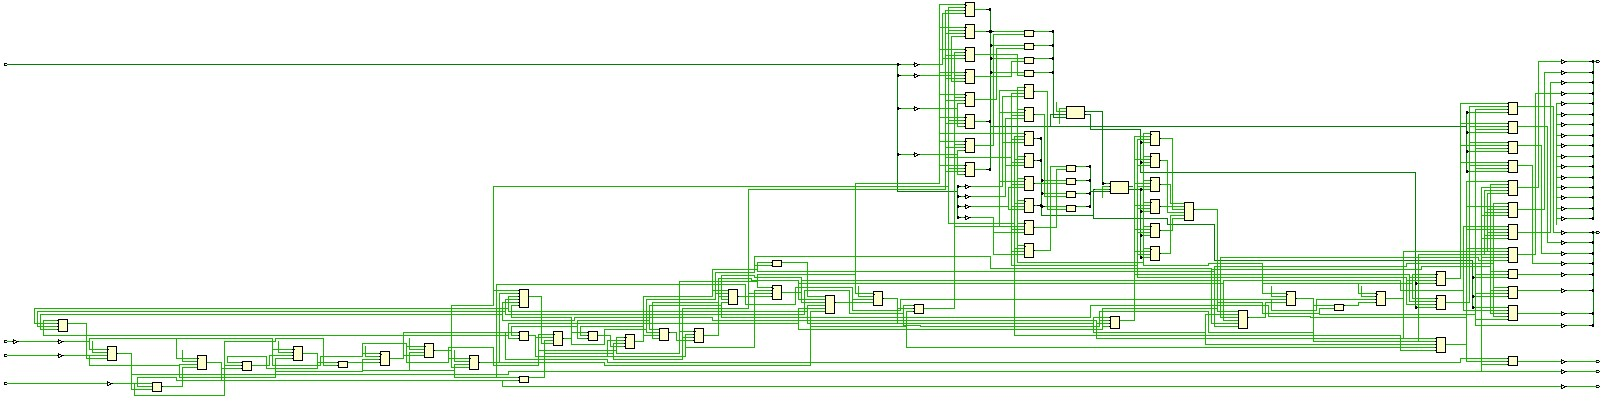
\includegraphics[scale=0.53,keepaspectratio]
			{schematic.jpg}}
		\caption{Schema sintetizzato}
		\label{schema}
	\end{figure}
\end{landscape}
	
	% Sezione per il testing

\section{Testing}
Per valutare la correttezza del componente sviluppato rispetto alle specifiche si \`e fatto uso di alcune serie di test di cui sono riportati alcuni esempi nella tabella a fine sezione. Il tempo \`e considerato da quando viene rilevata l'attivazione del segnale \texttt{i\_start} a quando viene attivato \texttt{o\_done} (In pratica il tempo impiegato per tornare a S0, valutato come numero di cicli di clock necessari).  

\subsection{Casi normali}
I tipi di test per questo tipo di esecuzione hanno seguito le modalit\`a dei testbench forniti (Esempi BT1 e BT2), valutando quindi sia casi di appartenenza a WZ sia casi negativi. I test effettuati hanno dato riscontri corretti sia in presintesi sia in postsintesi.

\subsubsection{Casi limite}
Per valutare il corretto funzionamento anche in casi limite sono stati realizzati testbench (Esempi BT3 e BT4) per cui l'indirizzo:
\begin{itemize}
	\item Appartenesse a WZ0 (Caso iniziale, con pipeline a regime);
	\item Appartenesse a WZ7 (Caso finale, nell'ultimo stato di analisi);
\end{itemize}
Per quanto riguarda invece le WZ, negli stessi esempi si sono testati casi di indirizzi base fuori ordine e al limite dei valori validi.
Tutti questi tipi di test sono stati eseguiti correttamente anche in postsintesi.

\subsection{Casi eccezionali}
Sono stati effettuati anche test in casi di esecuzione non normale per valutare la consistenza di comportamento del sistema.

\subsubsection{Esecuzioni con restart}
Sono stati effettuati test aggiungendo dei reset asincroni all'esecuzione dei benchtest gi\`a illustrati; prima dell'istruzione di \texttt{wait} per \texttt{tb\_done} \`e stato quindi inserito il seguente codice (con tempo di attesa variabile):
\begin{verbatim}
wait for 500 ns;
wait for c_CLOCK_PERIOD;
tb_rst <= '1';
wait for c_CLOCK_PERIOD;
tb_rst <= '0';
wait for c_CLOCK_PERIOD;
tb_start <= '1';
wait for c_CLOCK_PERIOD;
\end{verbatim}
\`E stata testata anche la possibilit\`a di esecuzioni multiple sequenziali senza reset ma con cambio di valori tra la terminazione del primo e lo start del secondo.

Dopo il restart i test sono stati completati correttamente, sia in presintesi sia in postsintesi. 

\subsubsection{Valori non validi}
Sono anche stati effettuatia alcuni test con valori non validi, al fine di controllare che le ipotesi effettuate in sezione \ref{eccezione} fossero corrette. Un esempio \`e mostrato dai test BT5 e BT6.

\subsection{Modifica del tempo di clock}
Come ultimi test sono stati diminuiti i tempi di clock delle simulazioni secondo quanto riportato nel report di sintesi. La simulazione postsintesi functional si comporta correttamente per i tempi di clock ipotizzati nel report di timing.

\begin{center}
	\begin{tabular}[width=\textwidth]{c|c c c c c c c c c|c|c}
		Test & 0 & 1 & 2 & 3 & 4 & 5 & 6 & 7 & 8 & Risultato & Nclock \\
		\hline
		BT1 & 4 & 13 & 22 & 31 & 37 & 45 & 77 & 91 & 33 & 180 (1 011 0100) & 9 \\
		BT2 & 4 & 13 & 22 & 31 & 37 & 45 & 77 & 91 & 42 & 42 (0 00101010) & 12 \\
		BT3 & 126 & 13 & 22 & 31 & 37 & 45 & 77 & 0 & 127 & 130 (1 000 0010) & 6 \\ 
		BT4 & 1 & 13 & 22 & 31 & 37 & 45 & 77 & 0 & 0 & 241 (1 111 0001) & 12 \\
		BT5 & 4 & 13 & 22 & 31 & 37 & 45 & 77 & 91 & 255 & 127 (0 1111111) & 12 \\ 
		BT6 & 4 & 13 & 22 & 31 & 37 & 45 & 77 & 254 & 255 & 226 (1 111 0010) & 12
	\end{tabular}
\end{center}

	
	% Sezione per le conclusioni

\section{Conclusioni}

Secondo la specifica fornita \`e stato possibile realizzare correttamente tramite descrizione in VHDL e successiva sintesi tramite Vivado un encoder di Working Zones. Il sistema \`e ottimizzato rispetto al tempo di esecuzione grazie all'uso della pipeline ed impiega tra 6 e 12 cicli di clock per fornire un output; il vincolo relativo al tempo di clock \`e rispettato ed \`e possibile un funzionamento in postsintesi con tempi fino a circa 4ns (functional).   


\end{document}